
\documentclass[letterpaper, reqno,11pt]{article}
\usepackage[margin=1.0in]{geometry}
\usepackage{color,latexsym,amsmath,amssymb}
\usepackage{fancyhdr}
\usepackage{amsthm}
\usepackage{mathtools}
\usepackage{tikz}
\usepackage{float}
\usepackage{centernot}
\usepackage{subcaption}
\usepackage{extarrows}
\usetikzlibrary{hobby}
\usetikzlibrary{shapes.multipart}
\usepackage{pgfplots}
\pgfplotsset{compat=1.7}
\usetikzlibrary{arrows.meta}

\newcommand{\RR}{\mathbb{R}}
\newcommand{\CC}{\mathbb{C}}
\newcommand{\ZZ}{\mathbb{Z}}
\newcommand{\QQ}{\mathbb{Q}}
\newcommand{\NN}{\mathbb{N}}
\def\upint{\mathchoice%
  {\mkern13mu\overline{\vphantom{\intop}\mkern7mu}\mkern-20mu}%
  {\mkern7mu\overline{\vphantom{\intop}\mkern7mu}\mkern-14mu}%
  {\mkern7mu\overline{\vphantom{\intop}\mkern7mu}\mkern-14mu}%
  {\mkern7mu\overline{\vphantom{\intop}\mkern7mu}\mkern-14mu}%
  \int}
\def\lowint{\mkern3mu\underline{\vphantom{\intop}\mkern7mu}\mkern-10mu\int}
\DeclareMathOperator{\card}{card}
\DeclareMathOperator{\Binomial}{Binomial}
\pagestyle{fancy}
\lhead{Math 321 Lecture 15}
\rhead{Yuchong Pan}
\begin{document}
\pagenumbering{arabic}
\title{Math 321 Lecture 15}
\author{Yuchong Pan}
\date{February 6, 2019}
\newtheorem{thm}{Theorem}
\newtheorem{defn}{Definition}
\newtheorem*{remark}{Remark}
\newtheorem{claim}{Claim}
\newtheorem{cor}{Corollary}
\newtheorem{lemma}{Lemma}
\newtheorem{prop}{Proposition}
\maketitle
%

\section{Riemann's Condition on Riemann-Stieltjes Integrability}

\begin{thm}
  \normalfont Let
  \begin{align*}
    f &: [a, b] \xrightarrow{\text{bounded}} \RR, \\
    \alpha &: [a, b] \to \RR \text{ be non-decreasing}.
  \end{align*}
  Then $f \in \mathcal R_\alpha[a, b]$ if and only if for every $\epsilon$, there exists a partition $P$ of $[a, b]$ such that $U_\alpha(f, P) - L_\alpha(f, P) < \epsilon$.
\end{thm}

\begin{proof}
  ``$\Rightarrow$'' Assume $f \in \mathcal R_\alpha[a, b]$. This implies that
  $$ \sup\{ L_\alpha(f, Q) : Q \text{ partition of } [a, b] \} = \inf\{ U_\alpha(f, Q) : Q \text{ partition of } [a, b] \} = \underbrace{\int_a^b fd\alpha}_{\int_a^b f(x) d\alpha(x)}. $$
  Fix $\epsilon > 0$.

  \begin{figure}[H]
    \centering
    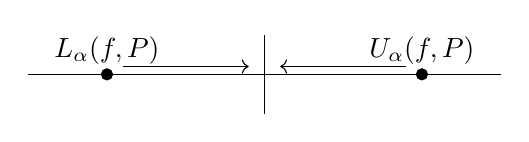
\begin{tikzpicture}
      \draw (-3, 0) -- (3, 0);
      \draw (0, -0.5) -- (0, 0.5);
      \draw[fill=black] (-2, 0) circle (2pt) node[above] {$L_\alpha(f, P)$};
      \draw[fill=black] (2, 0) circle (2pt) node[above] {$U_\alpha(f, P)$};
      \draw[->] (-1.8, 0.1) -- (-0.2, 0.1);
      \draw[->] (1.8, 0.1) -- (0.2, 0.1);
    \end{tikzpicture}
  \end{figure}

  Since a supremum is a least upper bound, therefore $\int_a^b fd\alpha - \frac{\epsilon}{2}$ is \emph{not} an upper bound for the set $\{ L_\alpha(f, Q) : Q \text{ partitions} [a, b] \}$; i.e., there exists a partition $Q_1$ such that
  $$ \int_a^b fd\alpha - \frac{\epsilon}{2} < L_\alpha(f, Q) \leq \int_a^b fd\alpha. $$

  \begin{figure}[H]
    \centering
    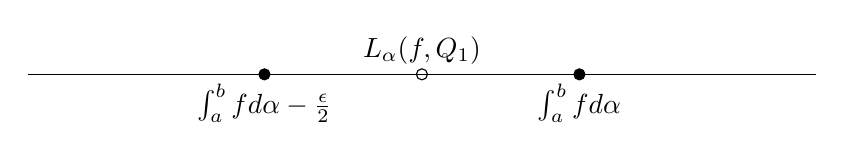
\begin{tikzpicture}
      \draw (-5, 0) -- (5, 0);
      \draw[fill=black] (-2, 0) circle (2pt) node[below] {$\int_a^b fd\alpha - \frac{\epsilon}{2}$};
      \draw (0, 0) circle (2pt) node[above] {$L_\alpha(f, Q_1)$};
      \draw[fill=black] (2, 0) circle (2pt) node[below] {$\int_a^b fd\alpha$};
    \end{tikzpicture}
  \end{figure}

  Similarly, an infimum is a greatest lower bound, so there exists a partition $Q_2$ such
  $$ \int_a^b fd\alpha + \frac{\epsilon}{2} > U_\alpha(f, Q_2) \geq \int_a^b fd\alpha. $$

  \begin{figure}[H]
    \centering
    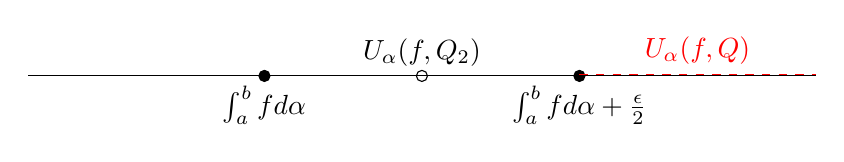
\begin{tikzpicture}
      \draw (-5, 0) -- (5, 0);
      \draw[fill=black] (-2, 0) circle (2pt) node[below] {$\int_a^b fd\alpha$};
      \draw (0, 0) circle (2pt) node[above] {$U_\alpha(f, Q_2)$};
      \draw[fill=black] (2, 0) circle (2pt) node[below] {$\int_a^b fd\alpha + \frac{\epsilon}{2}$};
      \draw[dashed, red] (2, 0.02) -- (5, 0.02) node[midway, above] {$U_\alpha(f, Q)$};
    \end{tikzpicture}
  \end{figure}

  \begin{figure}[H]
    \centering
    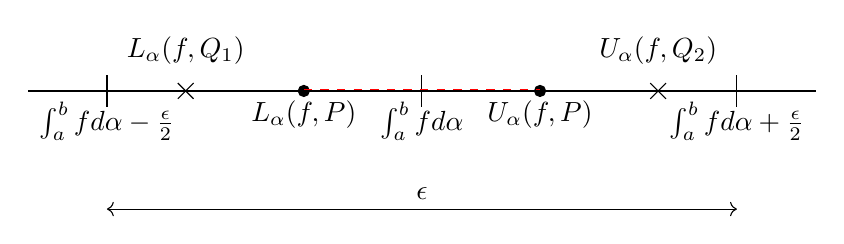
\begin{tikzpicture}
      \draw (-5, 0) -- (5, 0);
      \draw (0, -0.2) -- (0, 0.2) node[below, yshift=-6pt] {$\int_a^b fd\alpha$};
      \draw (-4, -0.2) -- (-4, 0.2) node[below, yshift=-6pt] {$\int_a^b fd\alpha - \frac{\epsilon}{2}$};
      \draw (4, -0.2) -- (4, 0.2) node[below, yshift=-6pt] {$\int_a^b fd\alpha + \frac{\epsilon}{2}$};
      \draw (-2.9, -0.1) -- (-3.1, 0.1);
      \draw (-2.9, 0.1) -- (-3.1, -0.1);
      \node at (-3, 0) [above, yshift=6pt] {$L_\alpha(f, Q_1)$};
      \draw (2.9, -0.1) -- (3.1, 0.1);
      \draw (2.9, 0.1) -- (3.1, -0.1);
      \node at (3, 0) [above, yshift=6pt] {$U_\alpha(f, Q_2)$};
      \draw[fill=black] (-1.5, 0) circle (2pt) node[below] {$L_\alpha(f, P)$};
      \draw[fill=black] (1.5, 0) circle (2pt) node[below] {$U_\alpha(f, P)$};
      \draw[dashed, red] (-1.5, 0.02) -- (1.5, 0.02);
      \draw[<->] (-4, -1.5) -- (4, -1.5) node[midway, above] {$\epsilon$};
    \end{tikzpicture}
  \end{figure}

  Set $P = Q_1 \cup Q_2 = \text{the common refinement of $Q_1$ and $Q_2$}$. We know that
  $$ L_\alpha(f, Q_1) \leq L_\alpha(f, P) \leq U_\alpha(f, P) \leq U_\alpha(f, Q_2). $$
  Since $U_\alpha(f, Q_2) - L_\alpha(f, Q_1) < \epsilon$, it follows that
  $$ U_\alpha(f, P) - L_\alpha(f, P) < \epsilon. $$

  $\Leftarrow$: Suppose that for every $\epsilon > 0$, there exists a partition $P$ of $[a, b]$ such that
  \begin{equation} \label{eq:*} \tag{*}
    U_\alpha(f, P) - L_\alpha(f, P) < \epsilon.
  \end{equation}
  \noindent {\bf Need to show:}
  \begin{equation} \label{eq:**} \tag{**}
    \sup_Q L_\alpha(f, Q) = \inf_Q U_\alpha(f, Q).
  \end{equation}
  \noindent {\bf Know:}
  $$ \text{LHS of \eqref{eq:**}} \leq \text{RHS of \eqref{eq:**}}. $$
  \noindent {\bf Remains to prove:}
  $$ \text{LHS of \eqref{eq:**}} \geq \text{RHS of \eqref{eq:**}}. $$

  \begin{figure}[H]
    \centering
    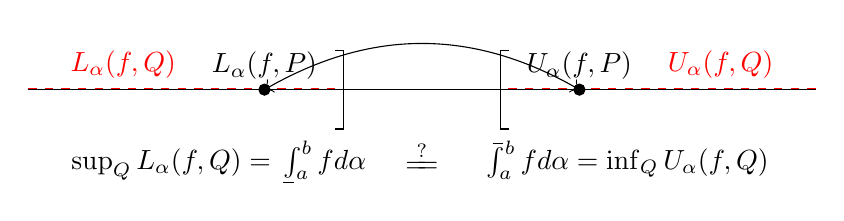
\begin{tikzpicture}
      \draw (-5, 0) -- (5, 0);
      \draw (-1.1, -0.5) -- (-1, -0.5) -- (-1, 0.5) -- (-1.1, 0.5);
      \draw (1.1, -0.5) -- (1, -0.5) -- (1, 0.5) -- (1.1, 0.5);
      \node at (-1, 0) [below, xshift=-45pt, yshift=-15pt] {$\sup_Q L_\alpha(f, Q) = \lowint_a^b fd\alpha$};
      \node at (1, 0) [below, xshift=45pt, yshift=-15pt] {$\upint_a^b fd\alpha = \inf_Q U_\alpha(f, Q)$};
      \node at (0, 0) [below, yshift=-15pt] {$\xlongequal{?}$};
      \draw[dashed, red] (-5, 0.02) -- (-1, 0.02) node[midway, above left] {$L_\alpha(f, Q)$};
      \draw[dashed, red] (5, 0.02) -- (1, 0.02) node[midway, above right] {$U_\alpha(f, Q)$};
      \draw[fill=black] (-2, 0) circle (2pt) node[above] {$L_\alpha(f, P)$};
      \draw[fill=black] (2, 0) circle (2pt) node[above] {$U_\alpha(f, P)$};
      \draw[<->, >={Classical TikZ Rightarrow[length=1mm]}] (-2, 0) to[bend left] (2, 0);
    \end{tikzpicture}
  \end{figure}

  Aiming for a contradiction, suppose $\lowint_a^b fd\alpha < \upint_a^b fd\alpha$; i.e.,
  $$ \upint_a^b fd\alpha - \lowint_a^b fd\alpha = d > 0. $$
  This means that
  $$ U_\alpha(f, P) - L_\alpha(f, P) \text{ for any partition $P$}. $$
  This contradicts our assumption \eqref{eq:*} if $\epsilon$ is chosen $< \delta$.
\end{proof}

\begin{remark}
  \normalfont ~
  
  \begin{center}
    \fbox{$U_\alpha(f, P) - L_\alpha(f, P) < \epsilon$}
    $$ \big\Downarrow $$
    $$ = \sum_{i = 1}^n \underbrace{(M_i - m_i)}_{\omega(f, I_i)} \underbrace{\Delta \alpha_i}_{\omega(\alpha, I_i)}. $$
  \end{center}
\end{remark}

\begin{defn}
  \normalfont Given any interval $I \subseteq [a, b]$, define
  \begin{align*}
    \omega(g, I) &= \text{{\bf maximum oscillation} of $g$ on $I$} \\
    &= \sup\{ g(x) - g(y) : x, y \in I \} \\
    &= \sup\{ g(x) : x \in I \} - \inf\{ g(y) : y \in I \}.
  \end{align*}
\end{defn}

\begin{remark}
  \normalfont
  \begin{itemize}
  \item If $g = f$ and $I = [x_{i - 1}, x_i]$, then $\omega(f, I_i) = M_i - m_i$.
  \item If $g = \alpha$ is non-decreasing, then $\omega(\alpha, I_i) = \alpha(x_i) - \alpha(x_{i - 1}) = \Delta \alpha_i$.
  \end{itemize}
\end{remark}

\begin{cor}
  \normalfont $C[a, b] \subseteq \mathcal R_\alpha[a, b]$ for \emph{any} non-decreasing $\alpha$.
\end{cor}

\begin{proof}
  We will use Riemann's condition. For every $f \in C[a, b]$, any non-decreasing $\alpha$ and any $\epsilon > 0$, we will find a partition $P$ of $[a, b]$ such that
  $$ U_\alpha(f, P) - L_\alpha(f, P) = \sum_{i = 1}^n \omega(f, I_i) \omega(\alpha, I_i) < \epsilon. $$
  $f$ is uniformly continuous, so there exists $\delta > 0$ such that
  \begin{equation} \label{eq:***} \tag{***}
    |x - y| < \delta \Rightarrow |f(x) - f(y)| < \frac{\epsilon}{\alpha(b) - \alpha(a)}.
  \end{equation}
  Choose
  $$ P = \{ a = x_0 < x_1 = a + \frac{\delta}{2} < x_2 = a + \delta < \ldots < x_n = b \}. $$
  Note:
  $$ \omega(f, I_i) < \frac{\epsilon}{\alpha(b) - \alpha(a)} ~ \forall i \text{ by \eqref{eq:***}}. $$
  Hence,
  \begin{align*}
    U_\alpha(f, P) - L_\alpha(f, P) &= \sum_{i = 1}^n \underbrace{\omega(f, I_i)}_{< \frac{\epsilon}{\alpha(b) - \alpha(a)}} \omega(\alpha, I_i) \\
    &< \frac{\epsilon}{\alpha(b) - \alpha(a)} \sum_{i = 1}^n \omega(\alpha, I_i) \\
    &= \frac{\epsilon}{\alpha(b) - \alpha(a)} \underbrace{\sum_{i = 1}^n (\alpha(x_i) - \alpha(x_{i - 1}))}_{= \alpha(b) - \alpha(a)} \\
    &= \epsilon.
  \end{align*}
\end{proof}

\begin{thm}
  \normalfont If $f_n, f \in \mathcal R_\alpha[a, b]$ and $f_n \xrightarrow{n \to \infty} f$ uniformly on $[a, b]$, then
  $$ \int_a^b f_n d\alpha \xrightarrow{n \to \infty} \int_a^b fd\alpha. $$
\end{thm}

\end{document}
